\documentclass[]{iac}
\usepackage{svg}
\usepackage{amsmath}
\DeclareMathOperator{\E}{E}
\DeclareMathOperator{\prob}{p}
\DeclareMathOperator{\tr}{tr}
\usepackage{caption}
\usepackage{subcaption}
\newcommand{\etalia}{\textit{et al.}}
\newcommand*{\vectornorm}[1]{\left\|#1\right\|}
\newcommand*\rfrac[2]{{{}^{#1}\!/_{#2}}} % running fraction with slash - requires math mode.
\newcommand*\T{\mathsf{T}}

\newcommand*{\ex}[1]{\textsuperscript{{#1}}}

\newcommand{\soppp}[1]{\mathbb{#1}}
	
\usepackage[acronym]{glossaries}

\makeglossaries

\newacronym{sar}{SAR}{Synthetic Aperture Radar}





\begin{document}
	\IACpaperyear{21}
	\IACpapernumber{B1,5,9}
	\IACconference{72}
	\IAClocation{Dubai, United Arab Emirates}
	%\IACcopyrightA{2021}{the authors}
	\title{Integrating Social Media and Remote Sensing Data for Flood Assessment in Developing Countries: A Case Study in Douala Estuary, Cameroon}
	
\IACauthor{Desire Muhire\ex{1,2},Swarnajyoti Mukherjee\ex{1,3},Krittanon Sirorattanakul\ex{1,4},Nzeussi Mbouendeu Charles-aimé\ex{1,5},Victor Hertel\ex{1,6},
Ikechukwu Maduako\ex{1,7},Chukwuma Okolie\ex{1,8},Daniela Vargas-Sanabria\ex{1,9},Lako Stephane\ex{1,10},Ikenna Arungwa\ex{1,11},Avanija Menon\ex{1,12},Abinash Silwal\ex{1,13},Alessandro Novellino\ex{1,14},Barthelemy Ndongo\ex{15},Marco Romero\ex{1,16}}{

\ex{1} Space Technology for Earth Applications (STEA) Project Group (PG), Space Generation Advisory Council (SGAC), Vienna, Austria\\
\ex{2} Department of physics, Chouaib Doukkali University, El Jadida, Morocco\\
\ex{3} Space System Engineer \& Business Professional, GP Advanced Projects, Srl, Brescia, Italy\\
\ex{4} Division of Geological and Planetary Sciences, California Institute of Technology, Pasadena, CA, USA\\
\ex{5} International Space University, 67400 Ilkirch-Graffenstaden; Strasbourg, France\\
\ex{6} IRS, University of Stuttgart, Germany\\
\ex{7} Department of Geoinformatics and Surveying, Faculty of Environmental Studies, University of Nigeria, Enugu Campus\\
\ex{8} Department of Surveying and Geoinformatics, Faculty of Engineering, University of Lagos, Nigeria\\
\ex{9} Laboratorio de Investigación e Innovación Tecnológica, Universidad Estatal a Distancia, Costa Rica\\
\ex{10} Climate and Water Resources Department, Water For Life Cameroon, Yaounde, Cameroon\\
\ex{11} Department of Surveying and Geoinformatics, School of Environmental Science, Federal University of Technology, Owerri, Nigeria\\
\ex{12} Department of Physics and Astronomy, University College London, United Kingdom\\
\ex{13} Department of Geomatics Engineering, Kathmandu University, Nepal\\
\ex{14} British Geological Survey, United Kingdom\\
\ex{15} Dschang University, Cameroon\\
\ex{16} Angolan Office for Space Affairs, Luanda, Angola
}


%%%%%%%%%%%%%%%%%%%%%%%%%%%%%%%%%%%%%%%%%%%%%%%%%%%%%%%%%ù	
	\abstract{According to the United Nations Office for Disaster Risk Reduction\cite{cred2015human}, the number of global weather-related disasters in the past decades has been estimated at 90\% of the total number of disasters. These are likely to increase in severity and frequency with current and forecasted global climate changes. Disaster risk monitoring using space technology and machine learning has become essential for minimizing and managing the consequences of natural disasters. However, flood assessment and data collection remain deficient in many parts of developing countries. Recent studies in Cameroon have identified socio-economic limitations and low adaptive capacity to manage floods that threaten and expose populations to vulnerability and danger. The increasing availability of smartphones and social media data allows individuals to directly document floods in real-time and otherwise poorly observed areas. However, these data are rarely used for flood assessment purposes in developing countries. This information, in synergy with remote sensing, can help disaster managers and rescuers determine routes and maps to support flood response as well as post-flood activities, such as calibrating flood hydrodynamic models. The paper will focus on integrating community social media with satellite remote sensing data to assess and assist in flood disaster emergency response and preparedness in Douala Estuary in Cameroon. \\
   \textbf{Keywords:} social media, disaster management, remote sensing, Cameroon
}
	
\maketitle

\section{Introduction}
Increasing Climate change will cause frequent natural disasters, human and material losses worldwide, and will severely affect developing countries. The number of global weather disasters during the period 1995-2015 is estimated at 90\% of the total number of disasters\cite{cred2015human}. During this period, floods affected 2.3 billion people worldwide, with more people affected in Asia and Africa than in other continents\cite{wahlstrom_human_2015}. 

Recent studies in northern Cameroon show that environmental factors, socio-economic constraints and lack of adaptability to flood management endanger and expose the population to vulnerabilities and risks\cite{bang_irony_2017,bang_evaluating_2019}. The international disaster database EM-DAT reports 16 floods in Cameroon between 1988 and 2017, which killed 131 people and affected nearly 400,000\cite{shen2019spatial}. The limited risk assessment is mainly due to the lack of institutions for flood prevention, immediate disaster protection and mitigation, and the financial capacity of highly trained personnel. However, the addition of data sources and big data can enable real-time flood assessment while significantly reducing costs\cite{ towe2020rethinking}. 

As demonstrated\cite{notti_potential_2018,panchal_flooding_2019}, open access satellite images widely used for flood monitoring may have some limitations (spatio-temporal resolution, visit time, etc.).  However, they can be complemented by auxiliary data. Communication via smartphones, social networks are emerging as reliable and inexpensive auxiliary data used by the scientific community for disaster assessment, especially floods \cite{le2016crowdsourced}. In emergencies, social media platforms such as Twitter have become a tool for exchanging information at the community level \cite{lacassin2020rapid}. Twitter can be used to improve the effectiveness of social reaction, awareness, and relief efforts when combined with existing crisis management methodologies, machine learning algorithms \cite{singh2019event} and supported community-level training \cite{carley2016crowd}. When satellite imagery is not available or if images are obscured by clouds, Twitter data can also provide real-time damage assessments of disaster situations providing advantages over other existing methods \cite{david2016tweeting, baranowski2020social}. 

This paper focuses on the use of Sentinel-1 Synthetic Aperture Radar (SAR) data in Douala, Cameroon to take advantage of its active illumination to obtain day/night and all-weather data and also seeks to use new auxiliary data based on social media which are very abundant on the continent, but not valued. 

The rest of the paper is organized as follows. Section 2 describes the study area while highlighting the anthropological causes of flooding in Douala. Section 3 presents the methods used to process radar images and social media data. Section 4 presents the results and Section 5 concludes with perspectives on actions to mitigate flooding in the region.	
\section{Study region}
Douala is the economic capital of Cameroon located at 04\textdegree03'N 9\textdegree41'E in Central Africa with a high population over 3 million inhabitants\cite{populationstatdouala2021}(Fig.\ref{fig:douala_city_map}). The problem of flooding is widespread in Cameroon\cite{bruckmann2019analyse,tangan2018community}. For instance, floods events have occurred up to 5-10 times a year in the capital and 1-5 times a year in rural areas such as Maga and Lagdo (Northern region)\cite{tangan2018community}. Since 1975, when the Bamendjin dam was constructed, the Ndop plain in northeastern Cameroon has experienced periodic flooding, especially during the rainy season\cite{sighomnou2005cameroon}. Limbe, a seaside town in the southwest region of Cameroon, was also heavily flooded in 2001, with over 2000 people homeless, and destroyed properties and infrastructure\cite{ngalim2020stakeholders}. In 2008, the geographical area of Nkolbisson, Cameroon, for example, was hit by two catastrophic floods\cite{bruckmann2019analyse,tangan2018community}. 
\begin{figure}[hbt!]
	\centering
	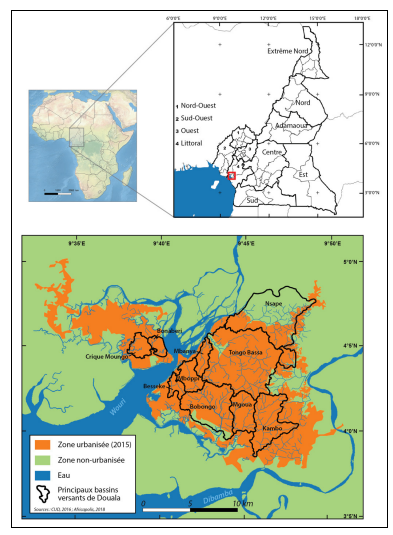
\includegraphics[width=0.8\linewidth]{figure/douala_city_map.png}
	\caption{Location of the urban area and the main watersheds of Douala. (Source: Figure 5 from \cite{bruckmann2019analyse})}
	\label{fig:douala_city_map}
\end{figure}

\subsection{Flood triggering mechanisms in Cameroon}

Poor waste management has been identified as a major cause of flooding in developing countries like Cameroon\cite{barthelemy2016legislative}. In Mefou, in central Cameroon and in the Dakar district of Douala (Fig.\ref{fig:dechet}), drains were observed to be clogged with plastic bottles and other solid waste\cite{gideonrole}. In another study by \cite{wung2019enhancing}, flooding in Limbe was discovered to be resulted from river channel blockage caused by indiscriminate dumping of refuse into the waterway and sediment deposition from upstream.

\begin{figure}[hbt!]
	\centering
	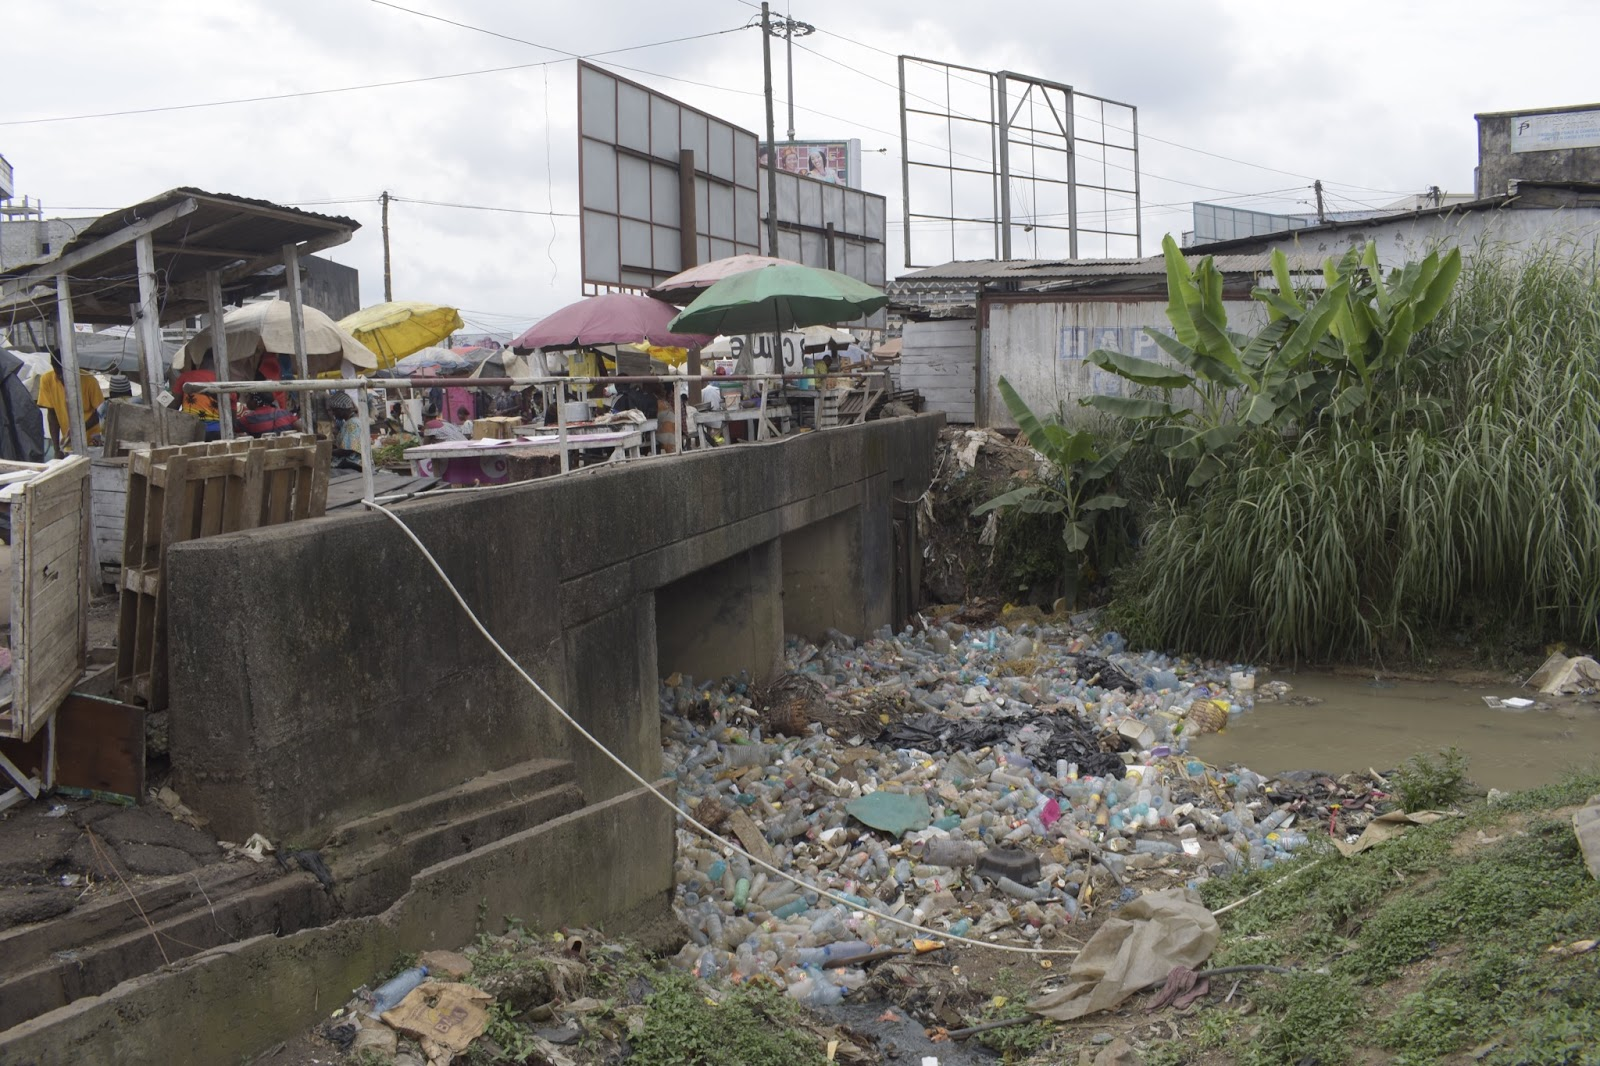
\includegraphics[height=4cm,keepaspectratio,width=0.8\linewidth]{figure/dechet.JPG}
	\caption{Plastic pollution completely blocking a waterway in the Dakar district of Douala, Cameroon\cite{greenpeaceorg}
}
	\label{fig:dechet}
\end{figure}

In the context of climate change, the increasing urbanization of the region is known to disregard drainage systems designed to contain runoff and the maximum volume of water that must flow through them during rainy periods. Thus, factors such as inadequate drains, uncontrolled waste disposal, and the nature of precipitation were considered common and important triggers to consider in mitigating and preparing for flooding in the region\cite{ngalim2020stakeholders}. 

\subsection{Precipitation in Douala}
In Douala, flooding is common during the rainy season from March to October(Fig.\ref{fig:douala_city_map} and \ref{fig:climateprecipitation}). The Tongo Bassa watershed located in the heart of the great Cameroonian economic metropolis of Douala, is one of the most affected urban location of the city. Tongo Bassa occupies an area of approximately 4200 ha or 42 $km^2$. The Tongo Bassa basin is crossed by three rivers and is characterized by a gentle slope (0.1 to 0.7\%) which exposes it to the daily tide variations. Bonamoussadi, Bepanda and Makepe Missoke are the most frequently affected areas, distributed on both sides of the Tongo Bassa river. 

\begin{figure*}[hbt!]
	\centering
	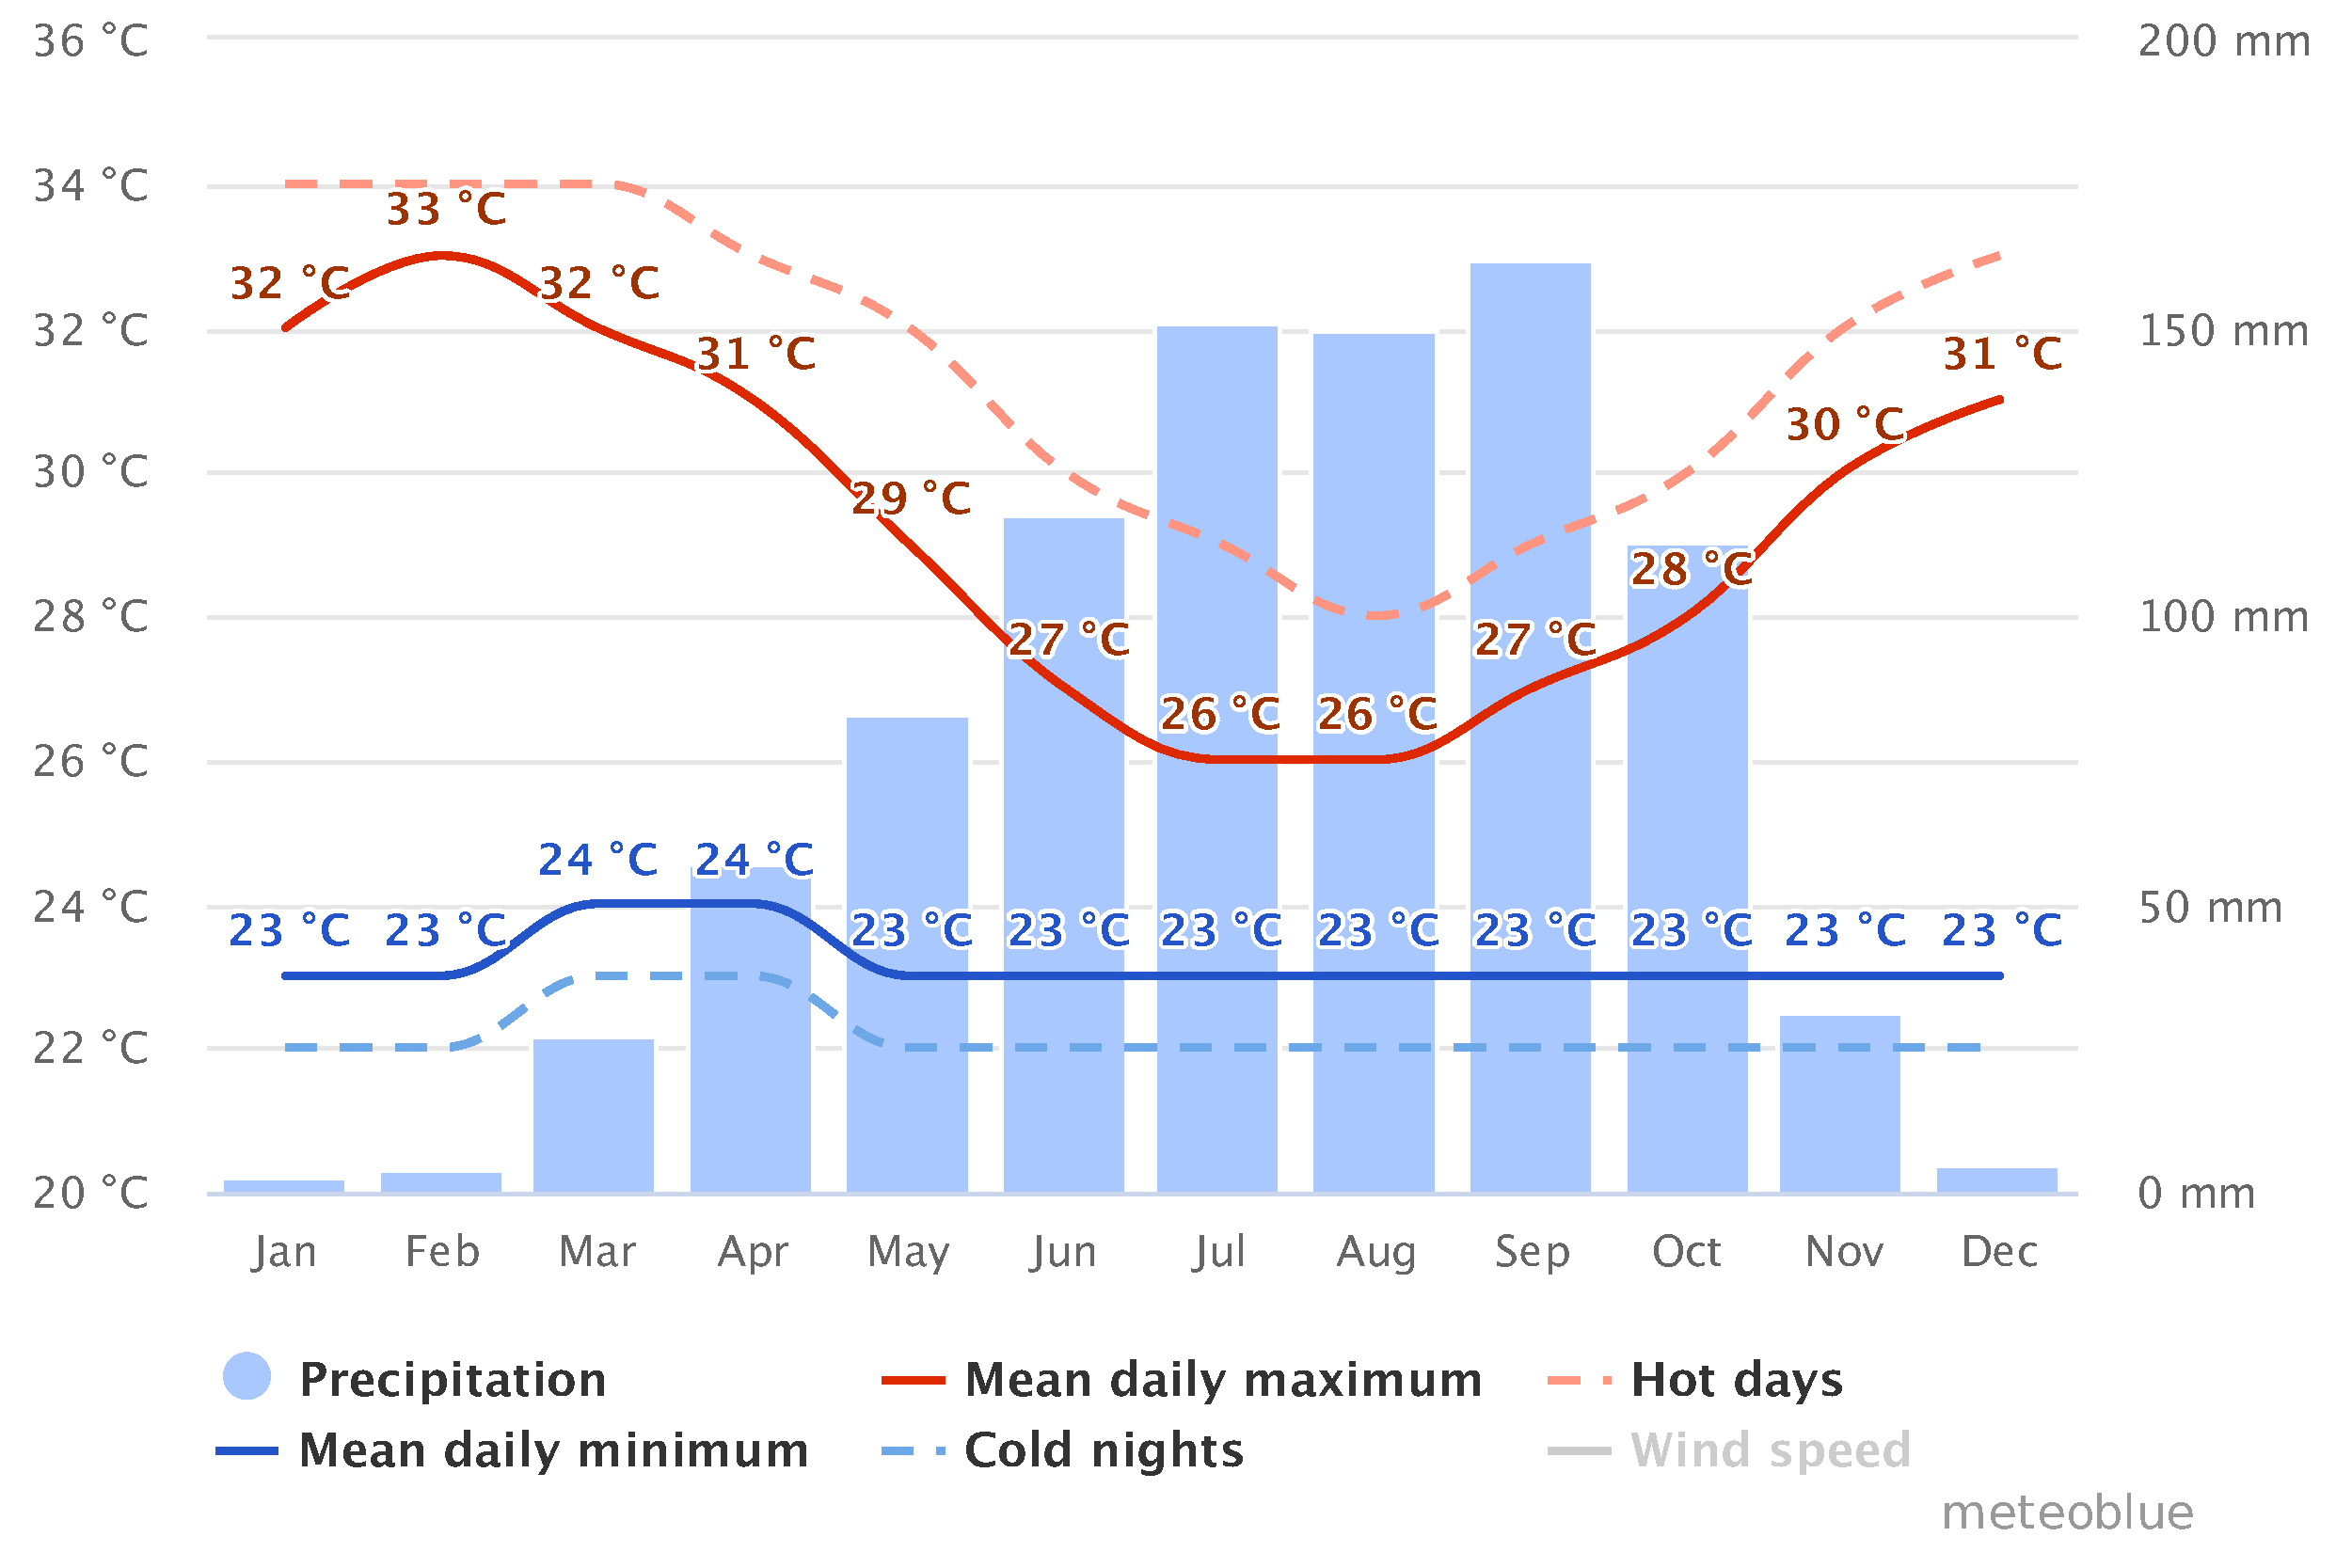
\includegraphics[width=0.5\linewidth]{figure/douala_climate.pdf}
	\caption{Douala Average temperatures and precipitation (Littoral, Cameroon, 4.05°N 9.7°E)(Source: www.meteoblue.com)\cite{meteoblue}. The mean daily maximum (solid red line) shows the maximum temperature of an average day for every month for Douala. Likewise, mean daily minimum (solid blue line) shows the average minimum temperature. Warm days and cool nights (dashed red and blue lines) show the average of the hottest day and coldest night of each month of the last 30 years}
	\label{fig:climateprecipitation}
\end{figure*}
\begin{figure}[hbt!]
	\centering
	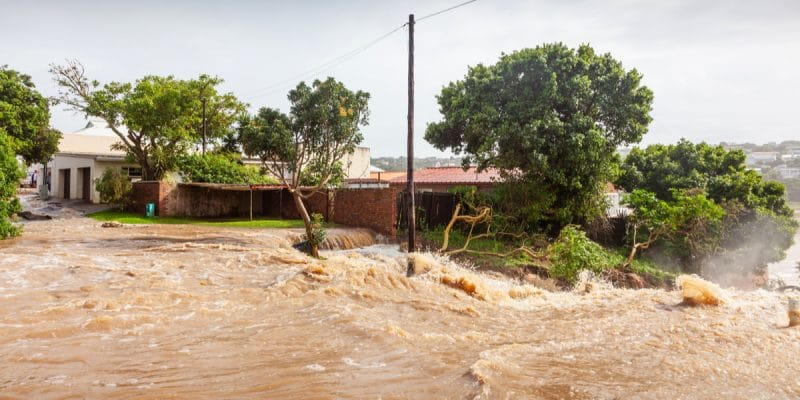
\includegraphics[width=0.8\linewidth]{figure/douala.jpg}
	\caption{Douala floods are frequents in July and August with several damage\cite{Afrik21}}
	\label{fig:floodimage}
\end{figure}

This highly urbanized basin is subject to rapid runoff towards low-lying areas with limited infiltration and high sedimentation rate in drains. Floods in these areas frequently affect residential houses, goods and services due to their exposure and low coping capacities of inhabitants, causing damage and loss of lives. This case is pertinent to the following dates: August 2\textsuperscript{nd} to 3\textsuperscript{rd}, 2000, August 9\textsuperscript{th}, 2010, and more recently that of August 21\textsuperscript{st}, 2020, August 11\textsuperscript{th}, 2021, September 1\textsuperscript{st}, 16\textsuperscript{th} and 18\textsuperscript{th} 2021.

\begin{figure}[hbt!]
	\centering
	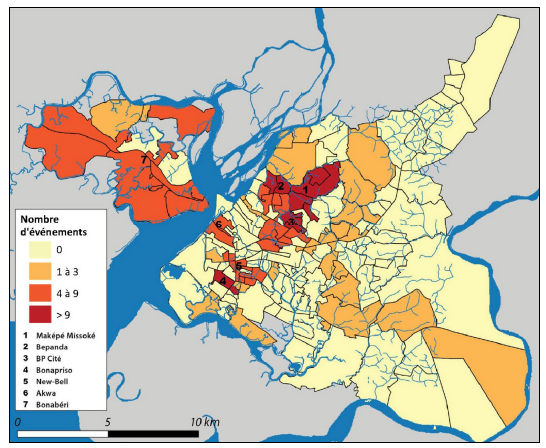
\includegraphics[width=0.8\linewidth]{figure/flood_distribution1984_2018.png}
	\caption{Spatial distribution of floods (31 events recorded) in Douala districts over the period 1984-2018. (Source: Figure 5 from \cite{bruckmann2019analyse})}
	\label{fig:flood_distribution1984_2018}
\end{figure}


\section{Methods}

\subsection{Synthetic Aperture Radar}
Synthetic Aperture Radar (SAR) is an active microwave remote sensing system in which a sensor sends a beam towards the ground and acquires the backscattered signals after interacting with the Earth's surface. Unlike optical satellite imagery, it is independent of solar electromagnetic energy and can capture high-resolution images during the day and night, in almost all-weather conditions, and through clouds \cite{Landuyt2019,WANG1995324}.

The scattering of objects on the SAR image is highly influenced by the terrain (geometry, features, etc.) and also acquisition properties (resolution, incident wave, ascending or descending-pass, etc.). In addition, the acquisition can be done by emitting and receiving horizontal (H) or vertical (V) polarization(cross-polarized (VH/HV) or co-polarized (HH/VV) acquisitions) that interacted differently with the ground. It therefore provides an additional information to characterize the phenomena of the observed region\cite{WANG1995324}. The best accuracy for flood mapping has been reported to be by using VH polarization configuration\cite{carreno2019flood}.

For a given mission of constant incidence angle and wavelength, the backscattering signal for a targeted area varies depending on the dielectric properties of the target, the physical shape of the scatterers in the target area of the resolution cell\cite{farr1993radar}. Water and metals represent objects with higher dielectric content than other materials and have a very large response. Therefore, if the geometric shape lies in front of the signal line of sight (such as the roofs of houses), the objects will appear bright because a strong signal is returned (or backscattered) to the sensor. On the other hand, if the surface is flat as a plane mirror, the incoming pulses reflect away from the sensor and they appear as a dark feature (flat water, etc.). Irregular geometries, such as vegetation cover, are grayed out because scattering occurs in all directions and only a small fraction of signals is reflected back to the sensor. Thus before flooding occurs, dry soil or vegetation would have a lower dielectric response. After an area has been flooded ,due to the high dielectric constant of water (80), the moisture content increases the returned signals. This response presents multiple reflections possibilities(specular reflection, double bounce, etc.) from the surface, which can make it difficult to extract the flood map, especially in vegetated (specular reflection or double-bounce within canopy) and urban areas (double bounce in buildings).

The SAR image has two major inherent limitations due to its angular viewing that leads to radiometric distortions or foreshortening and the diffraction induced speckle noises. SAR data exhibited salt and pepper noise are caused by a phenomenon inherent in the active coherent illumination system called speckles. These speckles are due to random constructive and destructive interferences in each resolution cell of the image, resulting in degradation of image quality and interpretation. Thus, before any application, these radar images must be pre-processed to remove the noises either by spatial filtering or by multi-looking operations\cite{argenti2013tutorial}.

In general, floods occur under severe weather conditions with heavy rainfall and dense cloud cover. These clouds hinder the effectiveness of optical satellite imagery\cite{sanyal2004}, hence, the use of SAR data for flood monitoring has become very common\cite{rao2006advantage}, and much research has demonstrated its effectiveness in flood events assessment \cite{martinez2007mapping}.

SAR-based flood detection techniques comprise thresholding-based methods \cite{Inglada2007}, image segmentation \cite{martinis2009towards}, statistical active contouring \cite{horritt2001flood}, rule-based classification \cite{pradhan2016new}, interferometric-SAR coherence analysis and data fusion approaches \cite{d2016bayesian}. 
To improve accuracy, thresholding-based flood detection techniques have evolved by merging additional data with the topographic data.


\subsection{Change detection}
The United Nations Platform for Space-based Information for Disaster Management and Emergency Response (UN-SPIDER) has made available an advanced thresholding-based method that generates flood extent map and assessment of affected areas\cite{un-spider}. 

The extent of a flood event is calculated using Sentinel-1 SAR data and a change detection method. This tool also includes an assessment of the number of people likely to be exposed, cropland and metropolitan areas affected, which can be cross-referenced with the generated flood extent layer and visualized in minutes.
This approach is suitable for developing countries as it uses the Google Earth Engine (GEE) cloud computing platform (https://code.earthengine.google.com) to process cloud-based remote sensing data. The main advantage is the speed of the computation, which is outsourced to Google's servers, as well as the availability of a variety of regularly updated datasets that are accessible directly in the code editor. Thus, it is possible to access the satellite data archive without having to download the raw data. The GEE GRD imagery includes the following steps: thermal noise removal, radiometric calibration, terrain correction. Therefore, only a speckle filter needs to be applied during pre-processing. 

A change detection approach was chosen, where images before and after the flood event are compared. This is due to the difficulties of detecting the city of Douala, which is mainly composed of vegetation and a dense urban area.  Using the basic histogram thresholding method, it is therefore difficult to distinguish flooded vegetation from urban flooding due to double-bounce backscatter\cite{manavalan2018review}.

Several supplemental datasets are used to suppress false positives in the flood extent layer. The European Commission's Joint Research Centre Global Surface Water dataset ('Source: EC JRC/Google', https://global-surface-water.appspot.com/) is used to mask all areas covered by water for more than 10 months per year with a spatial resolution of 30 m\cite{pekel2016high}. 

To eliminate pixels with slopes greater than 5\%, the Hydrological data and maps based on SHuttle Elevation Derivatives at multiple Scales (HydroSHEDS) digital elevation model of 3 Arc-Seconds was used. 
%\begin{figure*}[hbt!]
%	\centering
%	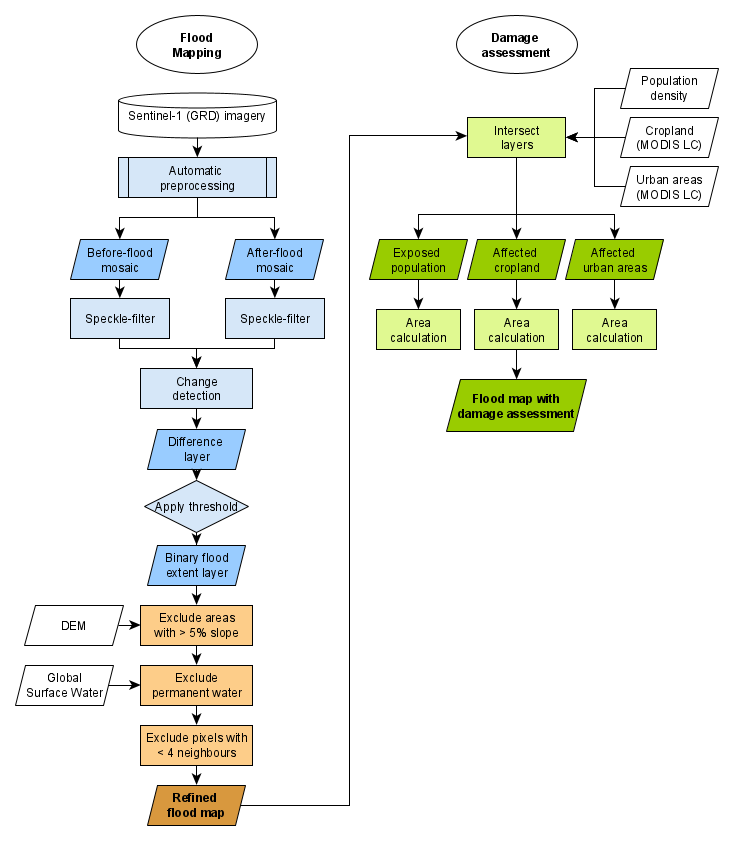
\includegraphics[width=0.6\linewidth]{figure/flood_mapping_GEE_workflow_1.png}
%	\caption{ The UN-SPIDER Recommended Practice workflow for flood mapping and damage assessment using Sentinel-1 SAR data in Google Earth Engine (Source:UN-SPIDER)\cite{un-spider}}
%	\label{fig:flood_mapping_GEE_workflow_1}
%\end{figure*}

\subsection{Sentinel 1}
Sentinel-1 is part of the space missions by the European Union and carried out by the European Space Agency (ESA) under the Copernicus program\cite{Panetti2014,geudtner2014sentinel}. This program aims to establish a global, continuous, autonomous, high quality and wide-range Earth observation capability. 

The constellation of polar-orbiting Sentinel-1 satellites (Sentinel-1A and Sentinel-1B) provides continuous SAR data day and night with a revisit time of 6 days. The data provided by the Copernicus Open Access Hub are mainly Single Look Complex (SLC) used for interferometry and the Ground Range Detected (GRD)\cite{filipponi2019sentinel}. Sentinel-1 Level 1 GRD products consist of focused SAR data that are multi-looked and projected to ground range using an Earth ellipsoid model. These data are accessible via the GEE and were used to map a flood event in August 2020, in Douala.
Sentinel-1 in the GEE are provided in different polarizations, modes, passes and resolutions\cite{ gees1}:
\begin{enumerate}
    \item Transmitter Receiver Polarization: ["VV"], ["HH"], ["VV", "VH"], or ["HH", "HV"]
    \item Instrument Mode: "IW" (Interferometric Wide Swath), "EW" (Extra Wide Swath) or "SM" (Strip Map). 
    \item Orbit Properties pass: "ASCENDING" or "DESCENDING"
    \item Spatial resolution meters: 10, 25 or 40
    \item GRD resolution: "M" (medium) or "H" (high).
\end{enumerate}
The Sentinel 1 satellite acquired were single polarization data at a spatial resolution of 5 m × 20 m, a 250 km swath width of view and in VH polarization.
\subsection{Twitter}

Publicly available tweets are retrieved by using python libraries snscrape (https://github.com/JustAnotherArchivist/snscrape). In this study, we used two different keywords in the query – "Cameroon flood" and "Cameroun inundation" (French for "Cameroon flood" ). For each tweet, we extract and retain the following information: tweeted time, content, number of replies, number of retweets, and number of likes. The tweets retrieved include both original tweets and replies, but not retweets. This work reports and discusses only aggregated statistics of the tweets.

To retrieve useful common terms and conduct sentimental analysis of the tweets, we need to pre-process the content of the tweets using techniques in Natural Language Processing. Natural Language Toolkit (NLTK) python library was used to perform the following steps:
\begin{enumerate}
    \item Remove links, mentions, and hashtag
    \item Splitting sentences into words and punctuation marks, or tokenization
    \item Remove stopwords such as articles, prepositions, and punctions that does not contribute to the meaning of the content
    \item Reducing the words into a root form or lemmatization, i.e. convert 2nd and 3rd forms of the verbs to the base verb
    \item Remove non-alphabetical characters and keep only words that contain three or more letters
\end{enumerate}

Using processed content from the tweets, we can determine the most common terms by using tf-idf vectorization. Term frequency of term t in document d is defined as:
\begin{equation}
tf(t,d)=n/N
\end{equation}

where n is the frequency of the term t in document d and N is the frequency of the term t in all documents in the database of the library used. The inverse document term frequency is given by:
\begin{equation}
tdf(t,d)=log(\frac{D}{d\in D: t \in D})
\end{equation}

where D is the total number of documents and ${d\in D: t \in D}$ represents the number of documents in which we find the term t. The product of term frequency and inverse document term frequency is called tf-idf. A more common term would have the tf-idf value of closer to zero. In our analysis, tf-idf vectorization using a machine learning python library, scikit-learn. Word clouds are then generated based on tf-idf values.

To conduct sentimental analysis, we use a python library Textblob. This library contains a trained models that could determine the polarity and subjectivity of a given text. Polarity ranges between -1 and 1 with positive values reflecting emotionally positive message and negative values reflecting emotionally negative messages. Those that are neutral would have polarity of 0. Subjectivity ranges between 0 and 1 with 1 being subjective and 0 being objective. Using both polarity and subjectivity would allow us to evaluate the sentiments of twitter users toward flooding issues in Cameroon.
	


\section{Results and Discussions}
The combination of several tools can significantly contribute to contribute to addressing this issue in developing and underdeveloped countries. developing countries. One tool would be satellite imagery such as Synthetic Aperture Radar.

\subsection{Flood mapping}
The flood map was obtained by processing Sentinel-1 GRD data with the UN-SPIDER change detection method in the GEE tool. Prior to processing, four dates are provided for a collection of pre- and post-flood images (Tab.\ref{tab:collectionofimage}. From these dates, the GEE searches for available images according to the parameters namely the region of interest, the polarization and the satellite ascending pass. In our case of the flood study of August  8\textsuperscript{th}, 2020 in Douala, two images S1 of 2020-08-02 were used as the pre-flood and S1 2020-08-26 as the post-flood (Fig. \ref{fig:pre_post_flood}. We have privileged a common DESCENDING pass to avoid different geometric distortion due to the angle.
\begin{table}[hbt!]\centering
\caption{Four dates defining a collection of images before and after the flood}
\begin{tabular}{lll}
\hline
\textbf{}       & \textbf{Start} & \textbf{End} \\
\hline
\textbf{Before} & 2020-08-01     & 2020-08-19   \\
\textbf{After}  & 2020-08-21     & 2020-09-01  \\
\hline
\end{tabular}\label{tab:collectionofimage}
\end{table}

\begin{figure*} %[hbt!]
	\centering
	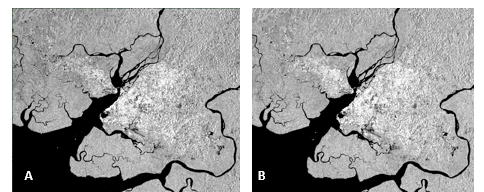
\includegraphics[width=5in]{figure/changedetection.png}
	\caption{Sentinel-1 imagery for flood analysis through UN-SPIDER change detection approach in Douala – (A) before, and (B) after flood event}

	\label{fig:pre_post_flood}
\end{figure*}

Figure \ref{fig:pre_post_flood} shows the before and after Sentinel-1 imageres which were subjected to the UN-SPIDER change detection approach for delineation of potentially flooded areas in Douala. 
The potentially flooded areas are displayed on higher resolution imagery in Figure \ref{fig:pre_post_flood}. Several flooded areas are observed along the banks of the Wouri River and along the channels of its tributaries (Fig. \ref{fig:flood_map}). From the imagery, the streams and tributaries within the floodplain exhibit a predominantly dendritic drainage pattern. In this pattern, there are no inner basins (endorheic drainage basins), and the floodplain is drained through the main drainage stem of the Wouri River and its tributaries. 

\begin{figure*} %[hbt!]
	\centering
	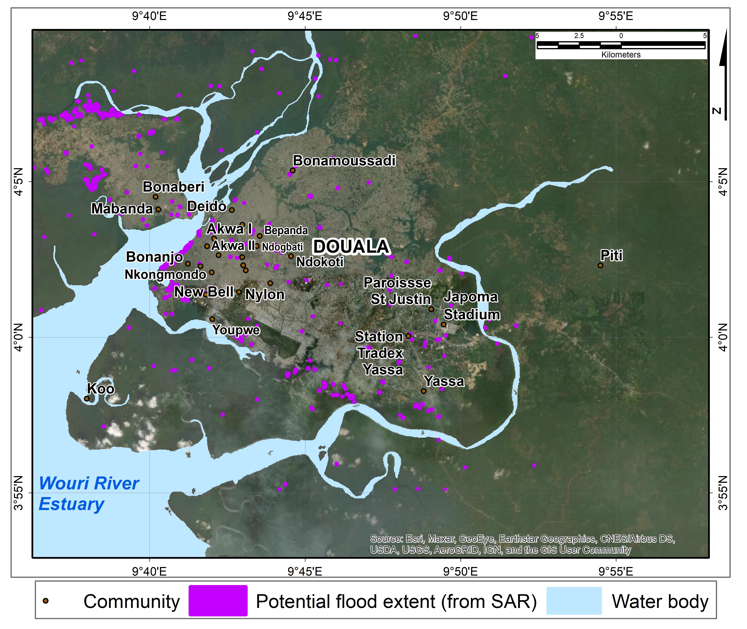
\includegraphics[width=0.45\linewidth]{figure/Douala_ops_1_IPCC_SAR_layA}
	\caption{Potential flood extent delineated from Sentinel-1 SAR processing (Imagery backdrop courtesy of ESRI Map service)}
	\label{fig:flood_map}
\end{figure*}

As a coastal city, Douala is also at risk of sea level rise (SLR) which has been identified by the United Nation’s Intergovernmental Panel on Climate Change (IPCC) as a threat to coastal cities. This is one of the combined factors leading to floods in Douala (Ndongo et al.,  2015). According to the IPCC in its Special Report on the Ocean and Cryosphere in a Changing Climate (SROCC), global mean sea levels will most likely rise between 0.95 feet (0.29m) and 3.61 feet (1.1m) by the end of the 21st century (IPCC, 2019). To portray the likely impact, the simulated water level from the 1.1m projected SLR was overlaid with the potentially flood areas from Sentinel-1 SAR in Figure 5.For validation of the SAR flood extent, a list of communities where flood incidents occurred in 2021\ref{fig:mbanya}).


\begin{figure*} %[hbt!]
     \centering
     \begin{subfigure}[b]{0.45\textwidth}
	\centering
	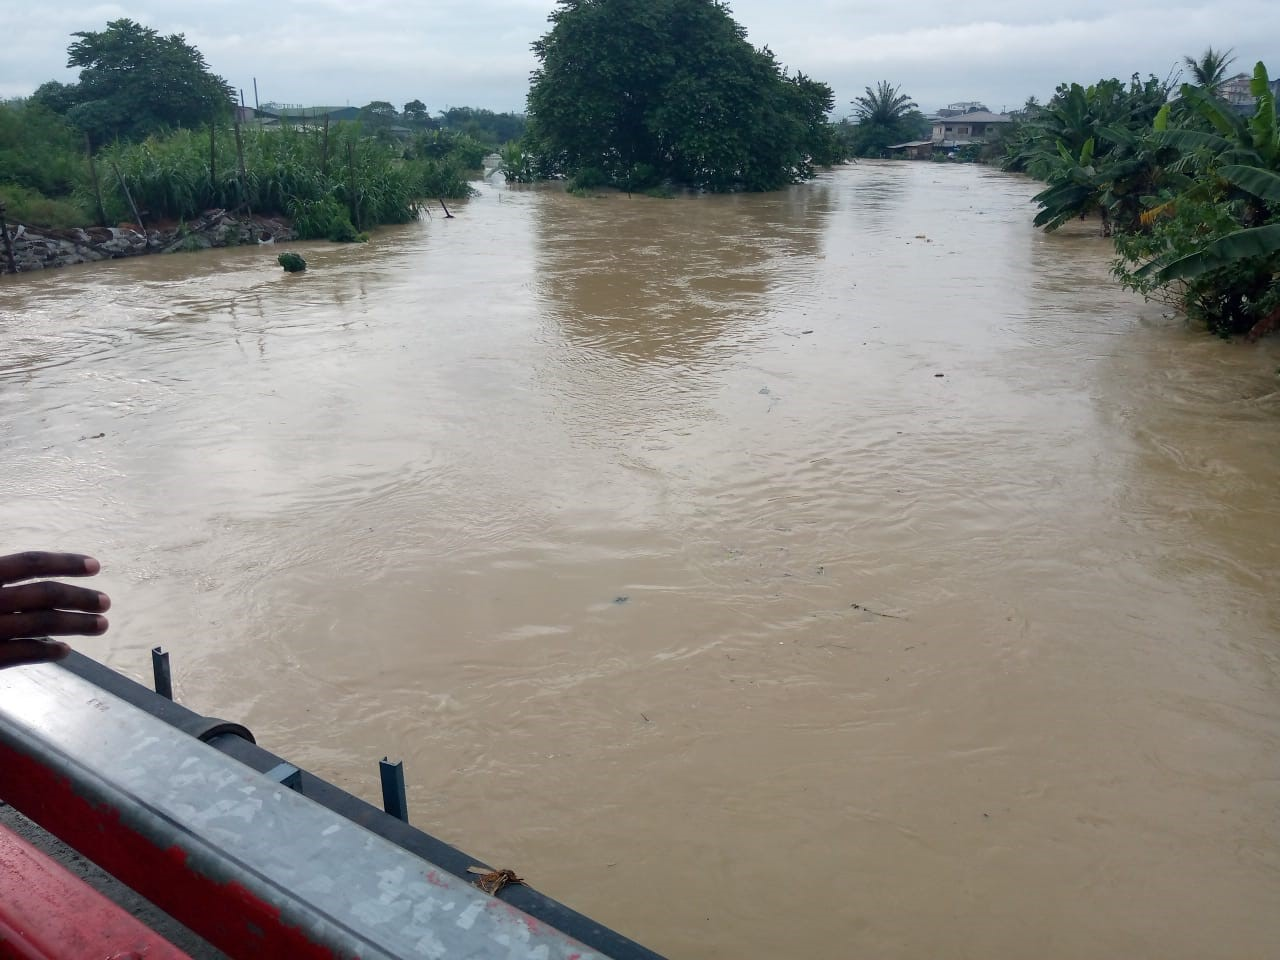
\includegraphics[width=0.8\linewidth]{figure/mbanya.jpg}
	\caption{}
	\label{fig:mbanya}
	\end{subfigure}
	 \hfill
     \begin{subfigure}[b]{0.45\textwidth}
	\centering
	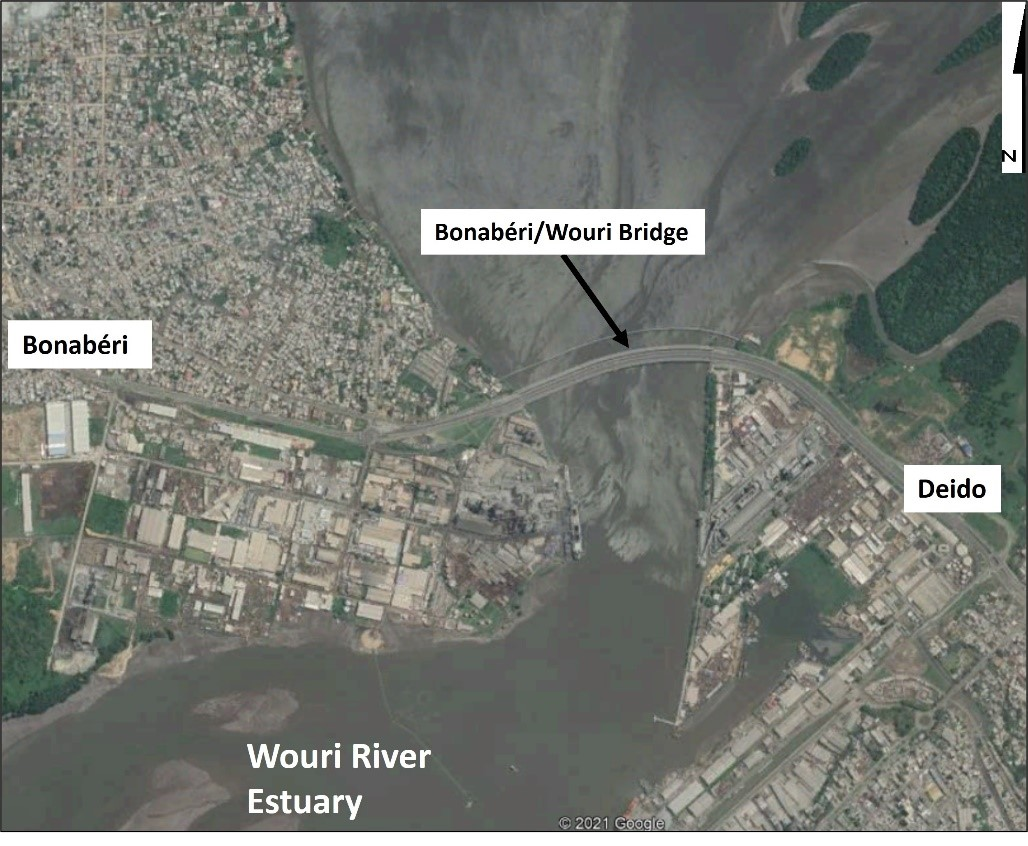
\includegraphics[width=0.7\linewidth]{figure/wouri_river.jpg}
	\caption{}
	\label{fig:wouri_river}
	\end{subfigure}
	\caption{A) Flooding in Mbanya, a community in Douala, September 16, 2021 
                (Source: Field survey, 2021); B) Channel constriction at a bridge crossing in the channel of the Wouri River}
                
\end{figure*}

With heavy flooding (e.g., the flooding in Mbanya community on 16 September 2021; Figure \ref{fig:mbanya}) there is the risk of overland flow causing collateral stream channels to emerge from some of the established tributaries. However some structural and non-structural measures have been put in place to protect the communities against fluctuating water levels and periodic flooding. 

The location of Douala at the south-eastern shore of the Wouri River estuary makes it particularly susceptible to flooding which could be exacerbated by storm surges and sea level rise (SLR). The river channel is flanked on either side by densely populated communities. Areas of concern are communities such as Bonaberi and Deido which are located close to a constriction around the Bonaberi/Wouri bridge along the channel of the Wouri River (see Figure \ref{fig:wouri_river}). Such constrictions could arise when confining margins occur on both sides of a channel at the same reach\cite{EnvironmentAgency2021}. Channel constrictions could instigate high velocity river flows which can rapidly diffuse into the surrounding flood plains and communities. 

Analysis of Figure \ref{fig:Dcamfloo} shows that several communities where actual flooding occurred in 2021 coincide with the potential flood extent delineated from Sentinel-1. Communities such as Mabanda, Bonaloka, Akwa, Bonanjo and Bali are either situated within or in very close proximity to the potential flood extents along the riverbanks. Some otheir neighbourhoods inland are also concerned by floods from sea level rise: bépanda, malangué, cite des palmiers. This is in line with restricted flow from tributaries existing inland. The simulated impact zones of the projected SLR are mainly along the banks of the Wouri River estuary. However, it is unclear how this could change in an extreme flood event or storm surge. Moreover, a more comprehensive analysis of the vulnerability of Douala to coastal flooding would involve consideration of both offshore and nearshore hydrodynamic forces such as tidal currents, wave action, winds, and ocean currents.  Other city architecture, dwellers waste management practices and meteorological factors would also enlighten the comprehension of flood mechanisms in Douala.
anjo.

\begin{figure*} %[hbt!]
	\centering
	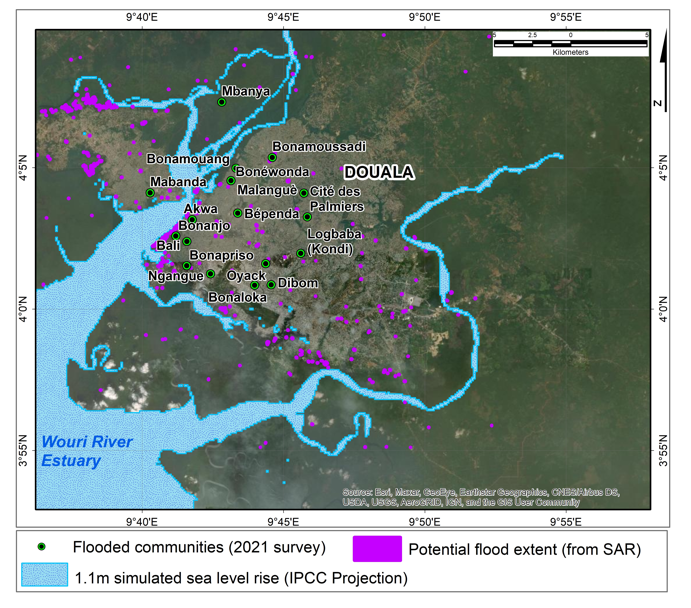
\includegraphics[width=0.45\linewidth]{figure/Douala_ops_1_IPCC_SAR_layB}
	\caption{Overlay of flooded communities and potential flood extent (between: 2020-08-21 and 2020-09-15) from Sentinel-1 SAR, with simulated impact of sea level rise in the Wouri River Estuary (Imagery backdrop courtesy of ESRI Map service)}
	\label{fig:Douala_ops_1_IPCC_SAR_layB}
\end{figure*}

\begin{figure*} %[hbt!]
	\centering
	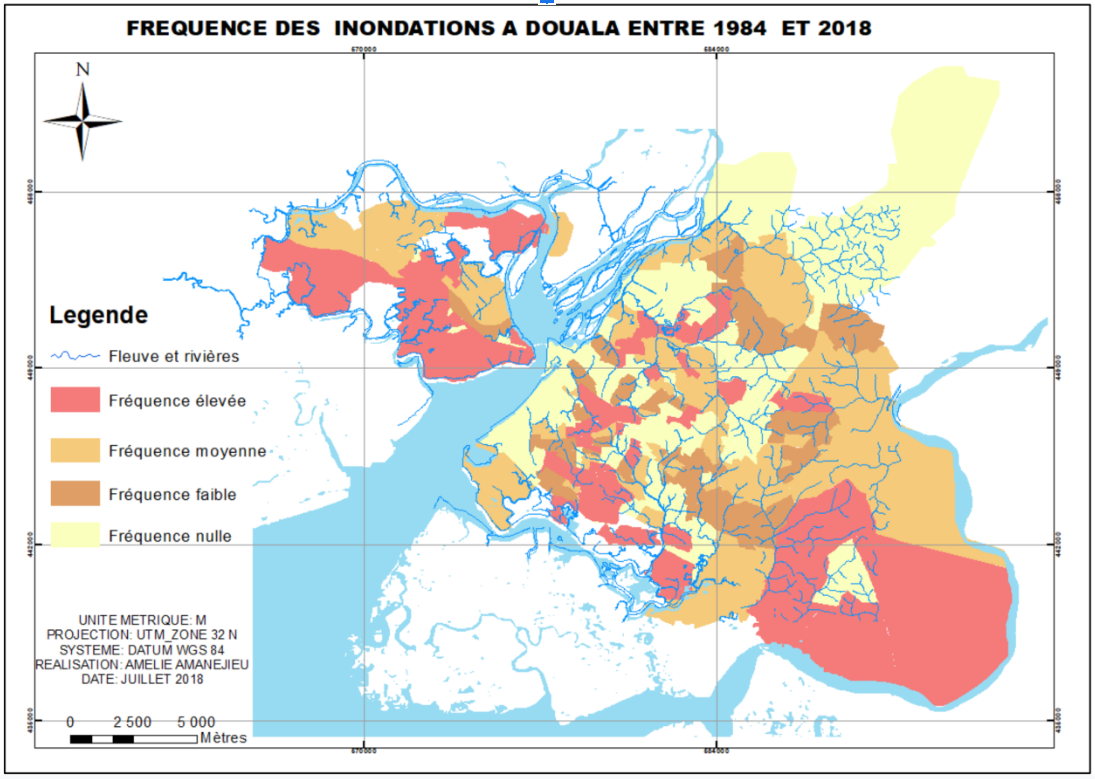
\includegraphics[width=0.45\linewidth]{figure/camfloo.PNG}
	\caption{Areas affected by floods between 1984 and 2018}
	\label{fig:Dcamfloo}
\end{figure*}

As a coastal city, Douala is also at risk of sea level rise (SLR) which has been identified by the United Nation’s Intergovernmental Panel on Climate Change (IPCC) as a threat to coastal cities. According to the IPCC in its Special Report on the Ocean and Cryosphere in a Changing Climate (SROCC), global mean sea levels will most likely rise between 0.95 feet (0.29m) and 3.61 feet (1.1m) by the end of the 21st century\cite{meredith2019polar}. To portray the likely impact, the simulated water level from the 1.1m projected SLR was overlaid with the potentially flood areas from Sentinel-1 SAR in Figure \ref{fig:Douala_ops_1_IPCC_SAR_layB}. 

The simulated impact zones of the projected SLR are mainly along the banks of the Wouri River estuary. However, it is unclear how this could change in an extreme flood event or storm surge. Moreover, a more comprehensive analysis of the vulnerability of Douala to coastal flooding would involve consideration of both offshore and nearshore hydrodynamic forces such as tidal currents, wave action, winds, and ocean currents.

Analysis of Figure \ref{fig:Douala_ops_1_IPCC_SAR_layB} shows that several communities where flooding occurred frequently coincide with the potential flood extent delineated from Sentinel-1. Communities such as Mabanda, Bonaloka, Akwa, Bonanjo and Bali are either situated within or in very close proximity to the potential flood extents along the riverbanks.
The simulated impact zones of the projected SLR are mainly along the banks of the Wouri River estuary. However, it is unclear how this could change in an extreme flood event or storm surge. Moreover, a more comprehensive analysis of the vulnerability of Douala to coastal flooding would involve consideration of both offshore and nearshore hydrodynamic forces such as tidal currents, wave action, winds, and ocean currents.

\subsection{Twitter analysis}
Between January 1st, 2010, and September 23rd, 2021, we are able to retrieve 4285 tweets with keyword “Cameroon flood” and 213 tweets with keyword “Cameroun inondation” (Figure \ref{fig:timeevolutioncumulation}). Dates with rapid increase in cumulative number of tweets are likely related to local flooding events. The largest outbursts for the number of tweets are in September 2012 and August 2015. The event in September 2012 seemed to be related to actual flood events in Cameroon, while the event in August 2015 was related to flood events in Nigeria as a resulting of water releases from a major dam in Cameroon. 

Analyzing the interactions between tweets using number of likes, number of retweets, and number of replies, we found that the interactions with each tweet vary over 3 orders of magnitudes. 95\% of all tweets have less than 5 likes, while the tweet with the largest number of likes has 778 likes. This reflects that some users have a much larger influence to the public that others.

Using tf-idf vectorization, we found the following words to be among the common words: “dam”, “Nigeria”, “releases”, “alert”, “water”, “issues”, “disaster”, “warning”, “kill”. We have also generated word clouds using the most common words for both keyword “Cameroon flood” and “Cameroun inundation” (Figure \ref{fig:Wordclouds}). 

\begin{figure}[hbt!]
	\centering
	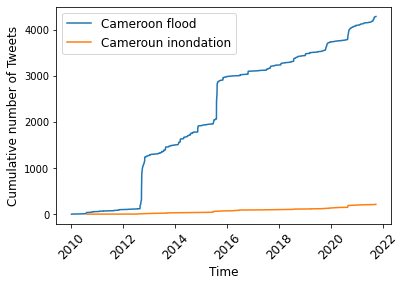
\includegraphics[width=0.8\linewidth]{figure/timeevolutioncumulation.png}
	\caption{Time evolution of the cumulative number of tweets retrieved using the keywords “Cameroon flood” and “Cameroun inondation”}
	\label{fig:timeevolutioncumulation}
\end{figure}

\begin{figure}[htp]
	\centering
	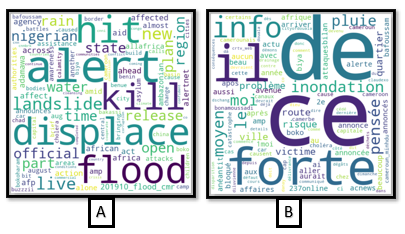
\includegraphics[width=0.8\linewidth]{figure/Wordclouds.png}
	\caption{Word clouds generated from content in the tweets retrieved using the keywords “Cameroon flood” (A) and “Cameroun inundation” (B)}
	\label{fig:Wordclouds}
\end{figure}


With the processed texts, the sentimental analysis reveals that about half of the tweets are neural in polarity. Among those that are not neural, 60\% shows positive polarity and 40\% shows negative polarity. In terms of subjectivity of the texts, we found an average subjectivity of 0.22 (see Figure \ref{fig:Sentimentalanalysis}). Since this value is closer to 0 than 1, this means that the texts are generally more objective than subjective. Since the content is generally more factual rather than opinions, it is not unexpected that the sentimental of the majority of tweets turns out to be closer to neutral.

We also manually analyzed the content in the tweets in French retrieved using the keyword “Cameroun inundation” between February 17 \textsuperscript{th}, 2018, and May 31\textsuperscript{st}, 2021. We found tweet content on 19 days that are related to flooding events in Douala, Cameroon (see Table \ref{table:twitteranalysis2020}). Among these, 4 days (July 25\textsuperscript{th}, 2018, August 21\textsuperscript{st}, 2020, August 22\textsuperscript{nd}, 2020, August 24\textsuperscript{th}, 2020) show significantly higher number of tweets per day. 

Most of the tweets on flooding events in Douala are almost evenly distributed among jokes, alert, sensitization and information. Some tweets are complaints (11\%) and very few calls to action mentioned (see Figure \ref{fig:twitteranalysis2020}). Floods from July 25th, 2020 , August 21st, 2020, and August 24th, 2020 recorded the highest number of tweets (5 to 14 tweets/day).
Analysis of the descriptive statistics of the tweets shows that in Cameroon, people are tweeting about floods, but the number of tweets is still very low compared to the statistics of tweets about other natural disasters in developed countries (e.g., hurricanes, floods, fires). Moreover, most of the tweets are not alerts or direct mentions on flood management. Therefore, there is a need to use social media more constructively so that an increasing number of Twitter users communicate about floods to improve flood predictability, registration, and response.


\begin{figure}[hbt!]
	\centering
	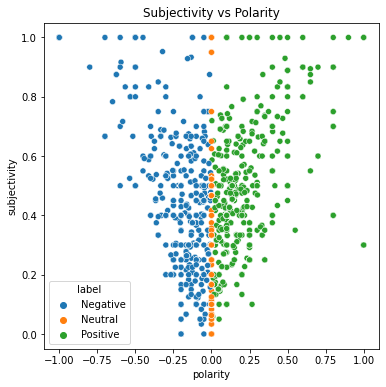
\includegraphics[width=0.8\linewidth]{figure/Sentimentalanalysis.png}
	\caption{Sentimental analysis of tweets with keyword “Cameroon floods”. The tweets are classified based on polarity as negative (polarity < 0, blue), neural (polarity = 0, orange), and positive (polarity > 0, green)}
	\label{fig:Sentimentalanalysis}
\end{figure}

\begin{table}[hbt!]\centering
\begin{tabular}{llll}
\hline
N° & Date       & N° & Date       \\
\hline
1  & 17/02/2018 & 11 & 04/09/2019 \\
2  & 04/03/2018 & 12 & 03/07/2020 \\
3  & 25/07/2018 & 13 & 21/08/2020 \\
4  & 26/07/2018 & 14 & 22/08/2020 \\
5  & 02/11/2018 & 15 & 24/08/2020 \\
6  & 30/06/2019 & 16 & 27/08/2020 \\
7  & 17/07/2019 & 17 & 04/09/2020 \\
8  & 07/08/2019 & 18 & 15/09/2020 \\
9  & 10/08/2019 & 19 & 31/05/2021 \\
10 & 23/08/2019 &    &  \\
\hline        
\end{tabular}
\caption{\label{table:twitteranalysis2020} Flood dates in Douala from Tweets record from February 2018 to may 2021}
\end{table}


\begin{figure}[hbt!]
	\centering
	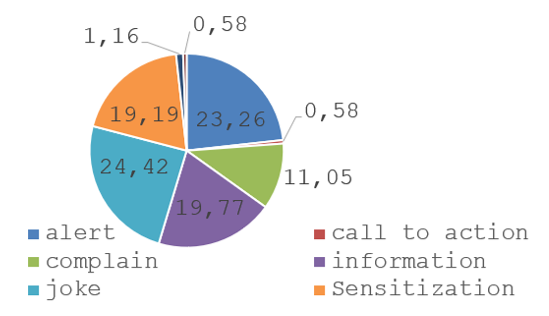
\includegraphics[width=0.8\linewidth]{figure/twitter_analysis_2020.png}
	\caption{Narrative of Twitter message screening in 2020}
	\label{fig:twitteranalysis2020}
\end{figure}




\section{Conclusion}
With climate change, floods natural disasters caused by storms and torrential rains are increasingly common and affect almost all populations and regions of the planet. In developing countries, managing these large-scale events is amplifying the socio-economic difficulties that these countries face. Flood maps are powerful disaster response planning tool for the immediate concern of human life, settlements and infrastructures. In this work, we used an open access tool which help in assessing the history of floods and the affected areas. In addition, we discuss the values, challenges, and possible advances of social networks use to leverage flood response strategies.

Twitter usage in Cameroon is still fairly limited compared to other developed countries. However, the data still allows us to learn about flood events that are not formally documented and associated sentiments from related individuals. Further analysis to compare twitter usage during flood events with regular scenarios would provide us with a better understand of how twitter and other social media can be adapted to assist with disaster managements, from early warning and mitigation to response and recovery.




\newpage
\bibliographystyle{unsrt} % We choose the &quot;plain&quot; reference style
\bibliography{refs}	
\end{document}